% !TEX program = lualatex
\documentclass[a4paper,11pt]{ltjsarticle}

\usepackage[haranoaji]{luatexja-preset}
\usepackage{fontspec}
\setmainfont{TeX Gyre Pagella}
\setsansfont{TeX Gyre Heros}
\setmonofont{Latin Modern Mono}[Scale=0.86,BoldFont={Latin Modern Mono}]

\usepackage[a4paper,top=25mm,bottom=24mm,left=22mm,right=22mm,headheight=28pt]{geometry}
\usepackage{amsmath,amssymb,mathtools}
\usepackage{booktabs,tabularx,longtable,array,multirow,colortbl}
\usepackage{enumitem}
\usepackage{xcolor}
\usepackage{graphicx}
\usepackage{tikz}
\usetikzlibrary{arrows.meta,positioning,fit,shapes.geometric,calc,backgrounds}
\usepackage[most]{tcolorbox}
\usepackage{listings}
\usepackage{xurl}
\usepackage{hyperref}
\usepackage{bookmark}
\usepackage{fancyhdr}
\usepackage{titlesec}
\usepackage{caption}
\usepackage{placeins}
\usepackage{lastpage}

\definecolor{TFNavy}{HTML}{102A43}
\definecolor{TFBlue}{HTML}{1261A0}
\definecolor{TFCyan}{HTML}{2CB1BC}
\definecolor{TFMint}{HTML}{D9F2F0}
\definecolor{TFGold}{HTML}{D69E2E}
\definecolor{TFRed}{HTML}{C53030}
\definecolor{TFGreen}{HTML}{2F855A}
\definecolor{TFInk}{HTML}{243B53}
\definecolor{TFMuted}{HTML}{627D98}
\definecolor{TFPaper}{HTML}{F8FAFC}
\definecolor{TFLine}{HTML}{CBD5E0}

\hypersetup{
  colorlinks=true,
  linkcolor=TFBlue,
  citecolor=TFBlue,
  urlcolor=TFBlue,
  pdftitle={TheoremForces White Paper},
  pdfauthor={TheoremForces Project},
  pdfsubject={A public certificate layer for reproducible Lean proofs},
  pdfkeywords={Lean, formal mathematics, reproducibility, certificate ledger, AI}
}

\pagestyle{fancy}
\fancyhf{}
\fancyhead[L]{\sffamily\small\color{TFMuted}TheoremForces White Paper}
\fancyhead[R]{\sffamily\small\color{TFMuted}Version 0.1.0 - 2026-08-07}
\fancyfoot[L]{\sffamily\footnotesize\color{TFMuted}Public beta design paper}
\fancyfoot[R]{\sffamily\footnotesize\color{TFMuted}\thepage\ / \pageref{LastPage}}
\renewcommand{\headrulewidth}{0.4pt}
\renewcommand{\headrule}{\hbox to\headwidth{\color{TFLine}\leaders\hrule height \headrulewidth\hfill}}

\titleformat{\section}
  {\sffamily\Large\bfseries\color{TFNavy}}
  {\thesection}{0.75em}{}
\titleformat{\subsection}
  {\sffamily\large\bfseries\color{TFBlue}}
  {\thesubsection}{0.65em}{}
\titleformat{\subsubsection}
  {\sffamily\normalsize\bfseries\color{TFInk}}
  {\thesubsubsection}{0.55em}{}
\titlespacing*{\section}{0pt}{2.2ex plus 0.6ex}{1.0ex}
\titlespacing*{\subsection}{0pt}{1.8ex plus 0.4ex}{0.7ex}

\setlist[itemize]{leftmargin=1.6em,itemsep=0.35em,topsep=0.4em}
\setlist[enumerate]{leftmargin=1.8em,itemsep=0.35em,topsep=0.4em}
\setlength{\parindent}{1em}
\setlength{\parskip}{0.32em}
\renewcommand{\arraystretch}{1.24}
\captionsetup{font=small,labelfont={bf,color=TFNavy}}

\newcolumntype{Y}{>{\raggedright\arraybackslash}X}
\newcolumntype{L}[1]{>{\raggedright\arraybackslash}p{#1}}
\newcommand{\term}[1]{\textbf{\color{TFNavy}#1}}
\newcommand{\status}[2]{\textcolor{#1}{\textbf{#2}}}

\newtcolorbox{principlebox}[1]{
  enhanced,breakable,
  colback=TFMint!42,colframe=TFCyan,
  boxrule=0.7pt,arc=2mm,
  left=3mm,right=3mm,top=2mm,bottom=2mm,
  title={#1},fonttitle=\sffamily\bfseries,coltitle=TFNavy
}
\newtcolorbox{warningbox}[1]{
  enhanced,breakable,
  colback=TFRed!4,colframe=TFRed!75,
  boxrule=0.7pt,arc=2mm,
  left=3mm,right=3mm,top=2mm,bottom=2mm,
  title={#1},fonttitle=\sffamily\bfseries,coltitle=TFRed
}
\newtcolorbox{decisionbox}[1]{
  enhanced,breakable,
  colback=TFBlue!4,colframe=TFBlue!80,
  boxrule=0.7pt,arc=2mm,
  left=3mm,right=3mm,top=2mm,bottom=2mm,
  title={#1},fonttitle=\sffamily\bfseries,coltitle=TFNavy
}

\lstdefinelanguage{Lean}{
  morekeywords={theorem,lemma,def,example,namespace,end,import,by,fun,forall,where,let,in,if,then,else,match,with,open,variable,structure,class,inductive,abbrev,exact,intro,rw,simp,have,show},
  sensitive=true,
  morecomment=[l]{--},
  morestring=[b]"
}
\lstset{
  language=Lean,
  basicstyle=\ttfamily\footnotesize,
  keywordstyle=\color{TFBlue}\bfseries,
  commentstyle=\color{TFMuted}\itshape,
  stringstyle=\color{TFGreen},
  backgroundcolor=\color{TFPaper},
  frame=single,rulecolor=\color{TFLine},
  framesep=5pt,xleftmargin=4pt,xrightmargin=4pt,
  breaklines=true,showstringspaces=false,
  columns=fullflexible,keepspaces=true
}

\begin{document}

\hypersetup{pageanchor=false}
\begin{titlepage}
\thispagestyle{empty}
\begin{tikzpicture}[remember picture,overlay]
  \fill[TFNavy] (current page.north west) rectangle ([yshift=-115mm]current page.north east);
  \fill[TFCyan] ([yshift=-115mm]current page.north west) rectangle ([yshift=-118mm]current page.north east);
  \foreach \x/\y/\r in {30/28/2.0,55/46/1.4,87/25/1.6,123/43/1.3,155/23/2.2,181/48/1.2}{
    \fill[TFCyan!65] ([xshift=\x mm,yshift=-\y mm]current page.north west) circle (\r mm);
  }
  \draw[TFCyan!55,line width=0.8pt]
    ([xshift=30mm,yshift=-28mm]current page.north west) --
    ([xshift=55mm,yshift=-46mm]current page.north west) --
    ([xshift=87mm,yshift=-25mm]current page.north west) --
    ([xshift=123mm,yshift=-43mm]current page.north west) --
    ([xshift=155mm,yshift=-23mm]current page.north west) --
    ([xshift=181mm,yshift=-48mm]current page.north west);
\end{tikzpicture}

\vspace*{17mm}
{\sffamily\bfseries\fontsize{15}{18}\selectfont\color{TFCyan} THEOREMFORCES}\par
\vspace{8mm}
{\sffamily\bfseries\fontsize{31}{38}\selectfont\color{white}
再現可能な Lean 証明のための\par
公開 certificate layer}\par
\vspace{5mm}
{\sffamily\fontsize{15}{20}\selectfont\color{white!83}
A Public Certificate Layer for Reproducible Lean Proofs}\par

\vspace{33mm}
\begin{tcolorbox}[
  colback=white,colframe=TFLine,boxrule=0.6pt,arc=2mm,
  left=5mm,right=5mm,top=4mm,bottom=4mm]
\textbf{Status}\quad Public beta design paper\hfill
\textbf{Version}\quad 0.1.0\hfill
\textbf{Date}\quad 2026-08-07

\medskip
本書は、TheoremForces の目的、trust model、certificate 仕様、judge architecture、
semantic provenance、security、governance、および 2026-2027 年の実行計画を示す。
実装済み機能と目標状態を明確に区別し、Lean acceptance を数学的 endorsement と
混同しないことを設計の中心に置く。
\end{tcolorbox}

\vfill
{\sffamily\large\bfseries\color{TFNavy}TheoremForces Project}\par
{\sffamily\color{TFMuted}\url{https://theoremforces.org/}}\par
\vspace{5mm}
{\footnotesize\color{TFMuted}
Independent project. Not affiliated with, endorsed by, or sponsored by Lean FRO,
the Lean project, or the mathlib maintainers.}
\end{titlepage}

\hypersetup{pageanchor=true}
\pagenumbering{roman}

\begin{tcolorbox}[
  colback=TFNavy,colframe=TFNavy,arc=2mm,
  left=5mm,right=5mm,top=4mm,bottom=4mm]
{\sffamily\bfseries\large\color{white}要旨}

\color{white!92}
TheoremForces は、人間と AI が作る Lean 4 の conjecture と proof body を、固定された
Lean / Mathlib 環境で検証し、その結果を再現・引用・再利用可能な certificate として
記録するための独立 platform である。中心的な問いは「誰が一番速く解いたか」だけではない。
何が、どの環境で、どの axiom と依存関係のもとに検証され、第三者がどこまで再現できるかである。

本書は certificate を単一の badge として扱わず、(1) kernel acceptance、
(2) artifact provenance、(3) active environment での reverification、
(4) informal intent review、(5) curation の五層に分ける。公開 beta の現状には、
外部利用、review quorum、artifact reconstruction、sandbox enforcement、toolchain migration に
未解決課題がある。したがって今後の優先順位は、機能拡張や課金ではなく、trust reset、
research lighthouse、external adoption、review network、条件付き monetization の順とする。
\end{tcolorbox}

\section*{Abstract}
TheoremForces is an independent platform for checking Lean 4 conjectures and proof bodies in a
pinned Lean / Mathlib environment and preserving the results as reproducible, citable, and reusable
certificates. The central question is not only who solved a problem, but exactly what was checked,
under which environment and axiom policy, with which certificate dependencies, and to what extent
an independent party can reproduce the result.

This white paper separates five assurance layers: kernel acceptance, artifact provenance,
reverification under the active environment, review of alignment with informal intent, and
mathematical curation. It documents both the public-beta system and a proposed target architecture.
The execution strategy is deliberately gated: repair trust-critical gaps first, demonstrate value
through real research collections second, grow a small retained external community third, and open
paid pilots only after reliability and operational thresholds are met.

\begin{decisionbox}{文書の読み方}
\begin{itemize}
  \item \term{Current}: 2026-08-07 時点で公開 UI、公開 API、公開 repository から確認できる状態。
  \item \term{Target}: 本書が提案する certificate schema v2 と production architecture。
  \item \term{Gate}: 次の phase へ進むための measurable exit condition。
  \item 本書は private web application と isolated judge source code の完全な security audit ではない。
\end{itemize}
\end{decisionbox}

\tableofcontents
\clearpage
\pagenumbering{arabic}

\section{問題設定}

\subsection{証明が生成される時代の provenance gap}

Lean は dependent type theory に基づく interactive theorem prover であり、elaborator や tactic が
生成した proof term は小さな kernel によって検査される\cite{leanref,leankernel}。この構造は、
tactic や AI が複雑化しても、最終的な formal derivability を kernel で確認できるという強い基盤を持つ。

しかし、kernel が受理したという事実だけでは、研究上必要な問いのすべてには答えない。

\begin{itemize}
  \item formal statement は、研究者が意図した informal theorem と一致しているか。
  \item proof はどの Lean / Mathlib revision と import set で検査されたか。
  \item \texttt{sorryAx}、custom axiom、compiler trust、既存 certificate への依存は何か。
  \item judge に投入された exact source と、後から UI が再構成する source は同一か。
  \item toolchain 更新後も通るか。通らない場合、historical validity と current compatibility をどう分けるか。
  \item AI が生成した artifact を、人間の review や数学的価値判断とどう区別するか。
\end{itemize}

TheoremForces は、この gap を certificate ledger と semantic provenance によって埋める。
目標は「AI が真理を宣言する platform」ではなく、「Lean が何を受理し、その artifact がどのように
作られ、何を意味すると人間が判断したかを分離して残す platform」である\cite{tfhome,tfsemantic}。

\subsection{対象ユーザー}

\begin{tabularx}{\linewidth}{L{34mm}YY}
\toprule
\textbf{利用者} & \textbf{主要 job} & \textbf{必要な assurance} \\
\midrule
数学者 & informal problem を Lean statement と proof project に分解する & intent alignment、citation、共同作業 \\
Lean formalizer & proof body を検査し、再利用可能な theorem chain を作る & exact environment、imports、axioms \\
AI theorem prover 開発者 & generated proof を外部 judge で評価し、benchmark record を残す & API、rate limit、machine-readable certificate \\
研究 group / lab & private work を保存し、公開時に選択的に certificate 化する & access control、export、migration \\
第三者 verifier & platform operator を全面的に信頼せず検算する & content address、manifest、one-command verifier \\
reviewer / curator & formal statement と数学的意図・価値を評価する & review trail、conflict policy、retraction \\
\bottomrule
\end{tabularx}

\subsection{非目標}

TheoremForces は mathlib の代替ではない。一般的で再利用可能な数学は、適切な review を経て
mathlib に upstream されるべきである。TheoremForces は、その前後で発生する conjecture、attempt、
pinned build artifact、AI disclosure、citation metadata を記録する staging / certificate layer である
\cite{tfabout,mathlib}。

また、Accepted は novelty、importance、peer review、publication readiness を意味しない。
Seeds は money、token、security、redeemable asset ではなく、platform 内の reputation signal に限定する。
marketplace、cash bounty、off-platform payment は scope 外である\cite{tfabout,tfpricing}。

\section{設計原則}

\begin{principlebox}{P1. Lean accepted は必要条件であり、数学的 endorsement ではない}
Kernel acceptance、artifact reproduction、intent review、curation を別々の state として表示する。
一つの緑 badge に統合しない。
\end{principlebox}

\begin{principlebox}{P2. Exact bytes over regenerated appearance}
証明書が hash する対象は、後日の template で再生成した表示ではなく、judge が実際に受け取った
byte-for-byte source と bundle である。表示も保存 artifact を source of truth とする。
\end{principlebox}

\begin{principlebox}{P3. Pinned is not latest}
Active pinned environment と upstream stable release は別の概念である。historical certificate は元の
epoch で再現し、current compatibility は migration campaign の結果として別記する。
\end{principlebox}

\begin{principlebox}{P4. Fail closed at trust boundaries}
Hash、dependency、axiom parse、resource limit、webhook identity のどれかを確認できない場合、
Accepted や fully reproducible と表示しない。未知を成功へ丸めない。
\end{principlebox}

\begin{principlebox}{P5. Public verification must not require operator trust}
Certificate JSON、artifact、manifest、Merkle inclusion proof、verifier を公開し、第三者が独立に
検算できる経路を用意する。SLSA provenance と in-toto attestation の考え方を参照し、何が、いつ、
どの builder と inputs から生成されたかを machine-readable に残す\cite{slsa,intoto}。
\end{principlebox}

\begin{principlebox}{P6. Research value before feature surface}
North Star は conjecture 総数や AI-generated submission 数ではない。外部利用者によって作られ、
別の proof または研究成果から再利用・引用された provenance-complete certificate 数である。
\end{principlebox}

\section{Assurance model}

\subsection{五つの独立した assurance layer}

\begin{figure}[htbp]
\centering
\begin{tikzpicture}[
  layer/.style={rounded corners=2mm,text width=137mm,minimum width=145mm,minimum height=12mm,draw=TFLine,thick,align=left,font=\sffamily\small},
  label/.style={font=\sffamily\bfseries\small,text=white,minimum width=29mm,minimum height=8mm,rounded corners=1.5mm},
  node distance=3mm
]
\node[layer,fill=TFPaper] (l1) {\hspace{33mm}\textbf{Kernel acceptance}\quad exact theorem term が recorded environment で type-check した};
\node[label,fill=TFBlue] at ([xshift=17mm]l1.west) {L1};
\node[layer,fill=TFPaper,below=of l1] (l2) {\hspace{33mm}\textbf{Artifact provenance}\quad source、bundle、environment、axiom、dependency の hash が完全};
\node[label,fill=TFCyan] at ([xshift=17mm]l2.west) {L2};
\node[layer,fill=TFPaper,below=of l2] (l3) {\hspace{33mm}\textbf{Reverification}\quad active environment または指定 migration epoch でも再検査済み};
\node[label,fill=TFGreen] at ([xshift=17mm]l3.west) {L3};
\node[layer,fill=TFPaper,below=of l3] (l4) {\hspace{33mm}\textbf{Intent review}\quad formal statement と informal intent の alignment を複数人が確認};
\node[label,fill=TFGold] at ([xshift=17mm]l4.west) {L4};
\node[layer,fill=TFPaper,below=of l4] (l5) {\hspace{33mm}\textbf{Curation}\quad 教育・研究・benchmark 上の価値を curator が選定};
\node[label,fill=TFNavy] at ([xshift=17mm]l5.west) {L5};
\end{tikzpicture}
\caption{一つの badge に畳み込まない assurance stack}
\end{figure}

L1 は Lean の kernel による derivability の確認である。L2 は、その確認対象と実行環境の provenance
を第三者が検算できることを表す。L3 は時間軸を導入し、historical acceptance と current compatibility
を分離する。L4 は人間が意図との一致を review した状態、L5 は数学的価値を選定した状態である。

この分離によって、たとえば次の表現が可能になる。

\begin{itemize}
  \item \status{TFGreen}{Lean accepted} / \status{TFRed}{artifact mismatch} / intent unreviewed
  \item \status{TFGreen}{Lean accepted} / provenance complete / \status{TFGold}{needs migration}
  \item Lean accepted / provenance complete / intent aligned / \status{TFNavy}{curated}
  \item Lean accepted / provenance complete / \status{TFRed}{intent misaligned} / useful accidental lemma
\end{itemize}

\subsection{Acceptance predicate}

Formal statement を $s$、proof body を $p$、direct certificate imports を $I$、generator version を $v$、
environment epoch を $E$、axiom whitelist を $W$ とする。生成 source と judge bundle を

\begin{align}
  A &= G_v(s,p,I,E),\\
  B &= \operatorname{Bundle}(A,I,E)
\end{align}

と定義する。$J_E(B)$ を isolated judge の結果、$X_E(A)$ を \texttt{\#print axioms} から得た
transitive axiom set、$D(B)$ を bundle から計算した direct dependency set、$H$ を SHA-256 とする。
新規 submission の Accepted 条件は、概念的には次である。

\begin{equation}
\begin{split}
\operatorname{Accept}(s,p,I,E) \iff {} & J_E(B)=\textsf{success} \\
& \land X_E(A)\subseteq W \\
& \land \texttt{sorryAx}\notin X_E(A) \\
& \land D(B)=I \\
& \land H(A)=h_A \land H(B)=h_B \\
& \land \operatorname{LimitsEnforced}(J_E).
\end{split}
\end{equation}

重要なのは、単なる process exit code 0 ではない点である。実行対象、axiom report、dependency、
resource policy、recorded hash が同一 transaction / attestation chain に結び付いて初めて L1 と L2 が成立する。

\subsection{Axiom policy}

Lean は definition が直接・間接に依存する axiom を \texttt{\#print axioms} で列挙する。
公式 reference は \texttt{sorryAx}、compiler trust、custom axiom と、標準的な
\texttt{propext}、\texttt{Classical.choice}、\texttt{Quot.sound} を区別している
\cite{leanaxioms,leanvalidate}。

TheoremForces の policy は次を満たすべきである。

\begin{enumerate}
  \item \texttt{sorryAx} は whitelist に関係なく hard reject。
  \item parse failure / missing report は success ではなく infrastructure failure。
  \item standard axiom、custom axiom、imported certificate constant を UI 上で別 category にする。
  \item certificate dependencies は axiom list の文字列推測ではなく、server-resolved bundle manifest から確定する。
  \item parser version と raw output hash を certificate に含める。
\end{enumerate}

\section{System architecture}

\subsection{Current public description}

公開 documentation によれば、web application は Next.js on Cloudflare Workers、database は Cloudflare D1、
Lean build は外部 isolated judge が担当する。web server 自身は Lean を実行せず、fixed namespace、
static filter、type-checking trailer、pinned toolchain、HMAC-authenticated callback を組み合わせる
\cite{tfabout,tfjudging,tfsecurity}。

公開 judge repository は Lean v4.13.0 と Mathlib v4.13.0 を pin し、GitHub Actions workflow で
targeted \texttt{lake build}、axiom whitelist enforcement、machine-readable axiom report を実装している
\cite{tfrepo}。一方、公開 submission は isolated arm64 worker を示しているため、public repository と
production topology の関係を architecture document で明示する必要がある。

\subsection{Target pipeline}

\begin{figure}[htbp]
\centering
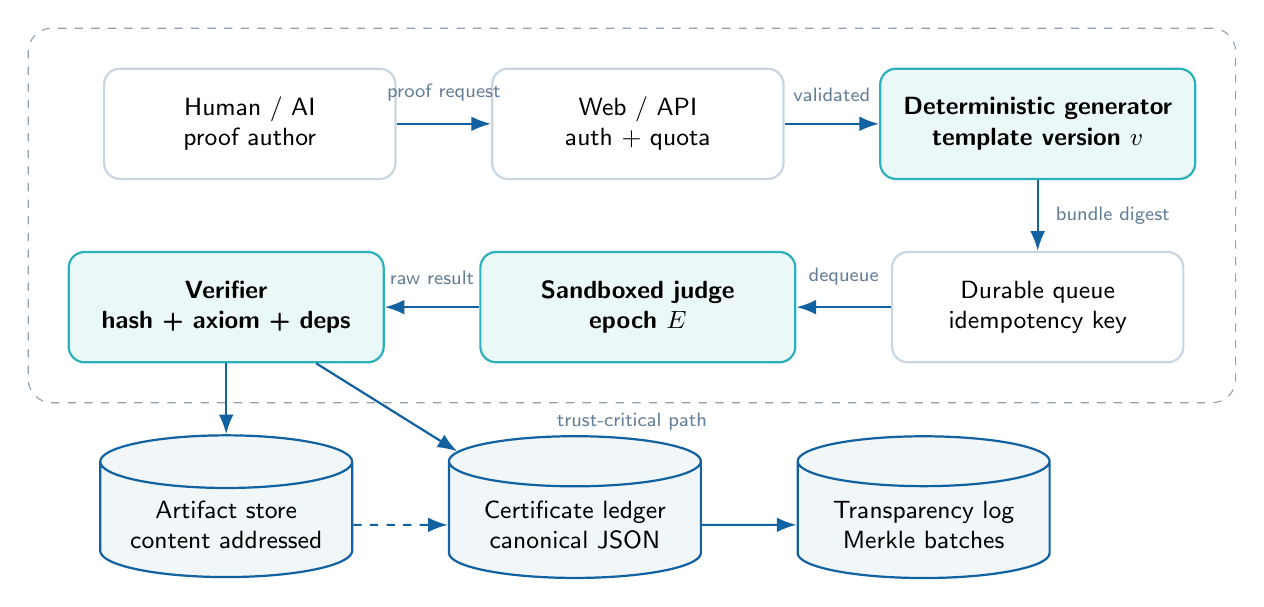
\begin{tikzpicture}[
  box/.style={rounded corners=2mm,draw=TFLine,thick,fill=white,minimum width=37mm,minimum height=14mm,align=center,font=\sffamily\small},
  trust/.style={rounded corners=2mm,draw=TFCyan,thick,fill=TFMint!55,minimum width=40mm,minimum height=14mm,align=center,font=\sffamily\small\bfseries},
  store/.style={cylinder,shape border rotate=90,aspect=0.25,draw=TFBlue,thick,fill=TFBlue!6,minimum width=32mm,minimum height=18mm,align=center,font=\sffamily\small},
  arr/.style={-{Latex[length=2.5mm]},thick,draw=TFBlue},
  note/.style={font=\sffamily\scriptsize,text=TFMuted,align=center},
  node distance=9mm and 12mm
]
\node[box] (author) {Human / AI\\proof author};
\node[box,right=of author] (app) {Web / API\\auth + quota};
\node[trust,right=of app] (gen) {Deterministic generator\\template version $v$};
\node[box,below=of gen] (queue) {Durable queue\\idempotency key};
\node[trust,left=of queue] (judge) {Sandboxed judge\\epoch $E$};
\node[trust,left=of judge] (verify) {Verifier\\hash + axiom + deps};
\node[store,below=of verify] (artifact) {Artifact store\\content addressed};
\node[store,right=of artifact] (ledger) {Certificate ledger\\canonical JSON};
\node[store,right=of ledger] (log) {Transparency log\\Merkle batches};

\draw[arr] (author) -- node[above=1.5mm,note]{proof request} (app);
\draw[arr] (app) -- node[above=1.5mm,note]{validated} (gen);
\draw[arr] (gen) -- node[right=1mm,note]{bundle digest} (queue);
\draw[arr] (queue) -- node[above=1.5mm,note]{dequeue} (judge);
\draw[arr] (judge) -- node[above=1.5mm,note]{raw result} (verify);
\draw[arr] (verify) -- (artifact);
\draw[arr] (verify) -- (ledger);
\draw[arr] (ledger) -- (log);
\draw[arr,dashed] (artifact) -- (ledger);

\begin{scope}[on background layer]
\node[fit=(gen)(queue)(judge)(verify),draw=TFNavy!45,dashed,rounded corners=3mm,inner sep=5mm,label={[note]below:trust-critical path}] {};
\end{scope}
\end{tikzpicture}
\caption{提案する end-to-end certificate pipeline}
\end{figure}
\FloatBarrier

\subsubsection{Submission intake}

Request は authenticated identity、conjecture id、proof body、AI disclosure、selected certificate imports、
client idempotency key を含む。server は quota と content-size cap を先に適用し、static filter の結果を
記録する。static filter は defense-in-depth であり、Lean soundness の完全な証明とは扱わない。

\subsubsection{Deterministic generation}

Generator は statement、proof body、server-resolved imports、namespace、type-checking trailer、axiom command を
順序を固定して出力する。生成 source は直ちに hash し、template version とともに immutable artifact store
へ保存する。後日の UI は source を再生成せず、この blob を表示する。

\begin{lstlisting}[caption={生成 artifact の概念例}]
-- generator: tf-wrapper-v2
-- environment: lean-4.32.2-mathlib-<commit>
-- submission: <id>

import Mathlib
import Theoremforces.Ledger.Cert_<dependency>

namespace Theoremforces.Conjectures.<NS>.Submissions.<ID>
<proof body bytes, unchanged>
def solution_target : <target type> := <answer name>
#print axioms solution_target
end Theoremforces.Conjectures.<NS>.Submissions.<ID>
\end{lstlisting}

\subsubsection{Sandboxed judge}

Judge image は digest で pin し、起動時 preflight で cgroup v2、network namespace、read-only base filesystem、
non-root uid、ephemeral workspace、PID / memory / CPU / wall-clock / output cap を確認する。
一つでも enforce できなければ production readiness check を失敗させる。

\subsubsection{Verification and minting}

Verifier は worker が返した status をそのまま信用しない。job identity、bundle hash、environment digest、
axiom report、dependency manifest、resource policy result を照合する。minting と public status update は
idempotent transaction とし、callback replay で二重 certificate や二重 reputation credit が発生しないようにする。

\subsubsection{Transparency log}

Certificate hash は UTC batch の Merkle tree に追加し、inclusion proof と signed tree head を公開する。
Merkle root を同一 database に保存するだけでは operator による履歴改変検出が弱いため、root を独立した
Git repository、release artifact、または別 provider の immutable storage に publish する。
RFC 9162 の transparency log は certificate domain は異なるが、append-only Merkle log の設計参照になる
\cite{rfc9162}。

\section{Certificate schema v2}

\subsection{Design goals}

v2 schema は「metadata がある」だけでなく、「第三者が同じ object graph を再構成できる」ことを目標とする。
SLSA が provenance を artifact の origin、time、builder、inputs に関する verifiable information と定義する
考え方を採り入れる\cite{slsa}。

\begin{tabularx}{\linewidth}{L{37mm}YY}
\toprule
\textbf{Object} & \textbf{Required fields} & \textbf{Verification purpose} \\
\midrule
Statement & canonical text, hash, conjecture id, intent revision & 何を証明したかを固定 \\
Proof body & exact bytes, hash, author disclosure & user input を固定 \\
Generated artifact & source blob digest, module path, template id & judge input の再構成を不要にする \\
Environment & Lean tag + digest, Mathlib commit, manifest hash, epoch & toolchain を同定 \\
Builder & image digest, architecture, sandbox policy, run id & 実行主体と制限を同定 \\
Axioms & normalized names, raw report hash, parser version & trust assumptions を監査 \\
Dependencies & direct / transitive cert hash, module hash, constant & graph と taint を追跡 \\
Result & exit status, timestamps, log digest, resource outcome & execution result を検算 \\
Transparency & batch id, leaf index, inclusion proof, signed root & append-only history を検算 \\
\bottomrule
\end{tabularx}

\subsection{Canonicalization}

Certificate payload $P$ は UTF-8、lexicographically sorted object keys、preserved array order、明示的 null policy を持つ
canonical JSON とする。certificate hash は自身の hash field を除いた canonical bytes に対して計算する。

\begin{equation}
  h_C = \operatorname{SHA256}(\operatorname{CanonicalJSON}(P \setminus \{\texttt{certificateHash}\})).
\end{equation}

Array order の意味を schema ごとに規定する。たとえば direct imports は request order ではなく canonical constant
で sort してよいが、Merkle audit path は順序を保持しなければならない。canonicalization implementation は
golden vectors を公開し、少なくとも二言語で同じ hash を生成することを test する。

\subsection{Lifecycle and supersession}

Immutable certificate を後から silent edit しない。問題が発見された場合は状態 record を append する。

\begin{itemize}
  \item \texttt{active}: 現在有効な historical acceptance record。
  \item \texttt{superseded}: 新しい environment / corrected provenance certificate が後継。
  \item \texttt{invalidated}: acceptance predicate または artifact integrity に重大な欠陥。
  \item \texttt{retracted}: informal explanation / authorship / policy 上の理由。kernel record は履歴として残す。
  \item \texttt{legacy-incomplete}: 過去 schema に必要 field がなく、完全再現を主張しない。
\end{itemize}

Status event 自体にも timestamp、reason code、actor、evidence link、previous event hash を持たせる。

\subsection{Independent verifier}

Reference CLI は次の UX を目標とする。

\begin{lstlisting}[language={},caption={目標とする verification UX}]
theoremforces verify tcl-cert-20260605-0d2nux

[ok] certificate canonical hash
[ok] statement and proof-body hashes
[ok] generated Lean source hash
[ok] judge bundle manifest
[ok] 4 direct certificate dependencies
[ok] Merkle inclusion proof
[ok] sandbox policy attestation
[ok] lake build in recorded environment
[ok] normalized axiom report matches certificate
\end{lstlisting}

Verification mode は三段階にする。

\begin{enumerate}
  \item \term{metadata}: download と hash / Merkle / dependency 検算だけ。
  \item \term{rebuild}: recorded container / toolchain で \texttt{lake build} を再実行。
  \item \term{migration}: selected target epoch で rebuild し、新しい compatibility report を作る。
\end{enumerate}

\section{Semantic provenance and review}

\subsection{なぜ kernel check と意味 review を分けるのか}

Lean kernel は formal statement の derivability を確認する。formal statement が informal theorem の翻訳として妥当か、
仮定が強すぎないか、定義が意図した対象を表すか、数学的価値があるかは別問題である。TheoremForces の公開 model は
Wild、Registry、Curated の三層を提案している\cite{tfsemantic}。

\begin{description}[style=nextline,leftmargin=1.5em]
  \item[Wild] AI-generated conjecture、failed attempt、scaffold、unreviewed certificate を探索として許容する。
  \item[Registry] Lean acceptance と machine-verifiable provenance を持つ record。数学的 endorsement ではない。
  \item[Curated] intent、axiom safety、essential dependencies、explanation、research / educational value を人間が確認する。
\end{description}

\subsection{Review dimensions}

Review を一票の like にしない。各 reviewer は少なくとも次を独立に評価する。

\begin{enumerate}
  \item \term{Intent alignment}: informal theorem と formal target が一致するか。
  \item \term{Assumption adequacy}: 不要に強い仮定、vacuous premise、empty type 依存がないか。
  \item \term{Definition fidelity}: custom definition が標準的数学概念を正しく表すか。
  \item \term{Dependency safety}: imported certificate の status と semantic role が適切か。
  \item \term{Explanation quality}: 数学者が proof の役割と限界を理解できるか。
\end{enumerate}

Canonical review status は reviewer eligibility、self-review exclusion、conflict of interest、blocking dispute、retraction を
考慮する。公開 documentation の 5 人 quorum は high assurance には妥当だが、初期 community では quorum が成立しにくい。
そのため UI は 0/5 を単なる未達として見せるだけでなく、各 dimension の partial progress と reviewer shortage を示す。

\subsection{AI disclosure}

AI 使用は許可し、acceptance を disclosure で差別化しない。ただし、human authorship、AI drafting、repair、autonomous submission
の level を machine-readable に記録する。reviewer は「AI を使ったか」ではなく、artifact、intent、dependency、explanation を評価する。

重要なのは、AI disclosure を proof validity の代用品にも、不正検出 detector にも使わないことである。自己申告は provenance の一部であり、
kernel acceptance は実際の Lean result、semantic endorsement は review record によって決まる。

\section{Security and abuse resistance}

\subsection{Threat model}

\begin{longtable}{L{31mm}L{49mm}L{68mm}}
\toprule
\textbf{Threat} & \textbf{Impact} & \textbf{Required controls} \\
\midrule
\endfirsthead
\toprule
\textbf{Threat} & \textbf{Impact} & \textbf{Required controls} \\
\midrule
\endhead
Fake acceptance & 証明なしで certificate / reputation を取得 & exact job identity、commit / bundle hash、verifier-side result fetch、idempotent mint \\
Namespace escape & 他 submission、statement、judge package を改変 & server-owned imports、wrapper namespace、token filter、minimal build context \\
Elaboration-time code execution & credential / filesystem / network 侵害 & no network、non-root、read-only root、seccomp、ephemeral workspace \\
Resource exhaustion & queue outage、費用増大、他 user の starvation & cgroup CPU / memory / PID、timeout、size cap、fair queue、quota \\
Axiom bypass & \texttt{sorryAx} や custom axiom を clean と表示 & semantic axiom report、fail-closed parser、raw report hash、regression corpus \\
Artifact substitution & 表示 source と judge source が不一致 & exact source blob、content address、bundle manifest、independent verifier \\
Dependency omission & imported theorem を base environment と誤表示 & server-resolved import manifest、direct/transitive closure check \\
Callback replay / confusion & 二重 credit、別 submission への結果付替え & HMAC、nonce / idempotency、submission + job + digest binding \\
Account takeover & private ledger / identity 侵害 & passkey / MFA、secure cookie、reset hardening、session revocation、audit log \\
Secret disclosure & infrastructure takeover & managed secret store、short-lived token、rotation、redaction runbook \\
Database compromise & private data exposure / ledger mutation & least privilege、encrypted backup、PII separation、external transparency root \\
Supply-chain compromise & judge image / action / dependency 改変 & digest pin、signed build provenance、dependency review、two-person release approval \\
\bottomrule
\end{longtable}

\subsection{Fail-closed resource enforcement}

Public sample logs observed on 2026-08-07 contain a warning that memory-limit capability was unavailable, while the job completed successfully
\cite{tfsample}. This observation does not by itself establish exploitability or root cause, but it is sufficient to define a P0 control:
production workers must refuse jobs when declared resource limits are not actually enforced.

\begin{warningbox}{Production invariant}
\texttt{LimitsEnforced = false} は warning ではなく infrastructure failure とする。
Proof failure、timeout、infrastructure failure、policy rejection を別 status にし、user に修正可能性を正確に伝える。
\end{warningbox}

\subsection{Secret handling and incident response}

Credential、VPN profile、invite link、service token を chat、Issue、commit、shared note に貼らない。secret manager と
short-lived credential を使用する。漏えいが疑われる場合は、削除より先に失効、scope 確認、access-log review、再発行、
incident timeline、再発防止を行う。operator account には MFA / passkey を必須とする。

\section{Public beta snapshot and trust reset}

\subsection{Snapshot: 2026-08-07}

公開 API と repository から確認した current snapshot は次の通りである\cite{tfstats,tfrepo,leanreleases}。

\begin{tabularx}{\linewidth}{L{54mm}L{35mm}Y}
\toprule
\textbf{Indicator} & \textbf{Observed value} & \textbf{Interpretation} \\
\midrule
Accepted certificates & 387 & supply は既に存在 \\
Distinct external accepted provers & 2 & external adoption は初期段階 \\
Reviewed certificates & 0 & semantic review network 未成立 \\
Curated certificates & 0 & curation 実績未成立 \\
No-disallowed-axiom rate & 95.1\% (368/387) & policy metric は存在、category audit が必要 \\
Active pinned environment & Lean / Mathlib v4.13.0 & historical reproducibility を保持すべき \\
Upstream stable Lean & v4.32.2 & active と latest を分離表示すべき \\
Open Issues / PRs in public judge repo & 0 / 0 & public feedback / roadmap 導線が弱い \\
Public pricing & beta、paid disabled & monetization より reliability gate が先 \\
\bottomrule
\end{tabularx}

\subsection{Observed trust gaps}

公開 sample submission では、UI が再計算した generated file hash と stored hash の不一致が表示される。また、その certificate では
environment epoch や lake manifest hash 等の provenance field が未記録の例がある\cite{tfsample,tfsamplecert}。
これは「proof が誤り」と即断する根拠ではないが、「表示された source が exact judge input であり、第三者が完全に再現できる」という
L2 claim を弱める。

さらに active pinned environment v4.13.0 に対し、公開 metric label は \textit{Reverified on latest Lean} と表現する。
2026-08-07 時点の upstream stable は v4.32.2 であるため、\textit{Reverified on active TheoremForces environment} と
\textit{Upstream version lag} に分ける方が正確である\cite{tfmetrics,leanreleases}。

\subsection{Trust reset plan}

\begin{enumerate}
  \item 新規機能と paid launch を一時 freeze。
  \item 全 387 certificate の artifact、dependency、environment、batch provenance を機械監査。
  \item \texttt{complete / legacy-incomplete / artifact-mismatch / dependency-mismatch / reverification-failed} に分類。
  \item mismatch / incomplete を fully reproducible と表示しない。
  \item exact generated source を immutable blob として保存・配信。
  \item schema v2 と verifier CLI を導入。
  \item sandbox limit preflight を fail closed に変更。
  \item v4.32.2 への shadow migration を実施し、failure taxonomy を公開。
  \item stats API を唯一の集計元にして page 間の counter / label を統一。
  \item public repository の branding、architecture、security policy、Issue workflow を現行化。
\end{enumerate}

\begin{decisionbox}{Trust reset exit gate}
新規 certificate の exact artifact hash、dependency record、sandbox enforcement が 100\% 一致し、restore drill が成功し、
public label inconsistency が 0、critical integrity incident なしで 14 日間運用できた時点で完了とする。
\end{decisionbox}

\section{Research workflow and interoperability}

\subsection{Flagship collection}

TheoremForces の価値は certificate 数ではなく、実研究の problem decomposition、proof reuse、citation に現れる。
flagship collection は最低限、次を一つの graph として提示する。

\begin{itemize}
  \item informal problem と paper / preprint / notebook の source
  \item formal target と intent mapping
  \item definition、auxiliary lemma、bridge lemma、target theorem の semantic role
  \item certificate dependency DAG
  \item exact reproducibility bundle
  \item AI assistance と human contribution disclosure
  \item known limitation、review status、migration status
  \item BibTeX / LaTeX / Markdown / JSON citation
  \item mathlib へ upstream すべき general-purpose component
\end{itemize}

初期候補は、公開 ledger に連鎖が見える Eisenstein integer / quadratic form 系列である。第二候補として、研究者が
実際に抱える inverse problem、geometry、analysis 等を選び、単発の toy problem と研究上の target theorem を区別する。

\subsection{Relationship to mathlib}

Mathlib は Lean 4 の shared mathematical library であり、source、cache、dependency workflow を公開している\cite{mathlib}。
TheoremForces は次の bridge を提供する。

\begin{enumerate}
  \item exploratory certificate から reusable lemma を特定する。
  \item dependency と axiom status を整理する。
  \item naming、generality、documentation、tests を mathlib contribution standard に合わせる。
  \item TheoremForces certificate を approval として扱わず、通常の mathlib review process へ提出する。
  \item upstream merge 後は、certificate の dependency を canonical mathlib theorem へ migration できるようにする。
\end{enumerate}

\subsection{Academic citation}

Citation は platform homepage ではなく immutable certificate version を指す。推奨 citation bundle は title、authors / attribution、
certificate id、certificate hash、formal statement hash、environment epoch、access date、permanent URL、related paper DOI を含む。
public attribution は privacy request により mutable であり得るため、certificate hash から個人情報を分離する。

\subsection{Preservation tiers}

\begin{itemize}
  \item \term{Online}: site、API、certificate JSON、source artifact。
  \item \term{Exportable}: self-contained tar / OCI bundle、manifest、verification script。
  \item \term{Replicated}: operator と異なる provider / Git repository に batch root と public artifacts を mirror。
  \item \term{Migrated}: historical epoch と active epoch の両方で status を追跡。
\end{itemize}

Reproducible Builds project が示すように、同一 source だけでなく、tool、environment、instructions を記録し、第三者が再実行して
artifact を比較できる経路が必要である\cite{reprobuilds}。

\section{Governance and sustainable operation}

\subsection{Small-team operating model}

TheoremForces は public documentation 上、single independent maintainer の hobby project であり SLA を持たない\cite{tfabout}。
この制約を隠さず、同時進行 epic を最大 2、weekly triage を 30 分、monthly roadmap review を 1 回とする。

\begin{tabularx}{\linewidth}{L{48mm}YY}
\toprule
\textbf{Area} & \textbf{Primary responsibility} & \textbf{Required second check} \\
\midrule
Research vision / flagship curation & mathematics lead & infrastructure feasibility \\
Judge / sandbox / observability & infrastructure lead & trust-policy review \\
Certificate schema / public claims & joint & two-person approval \\
Security incident & infrastructure lead & timeline and disclosure review \\
Academic outreach / case study & mathematics lead & participant consent \\
Paid pilot / legal entity & joint & gate review and external advice \\
\bottomrule
\end{tabularx}

\subsection{Change governance}

Trust-critical change は Issue、design note、tests、review、rollback plan、changelog を必要とする。特に次は two-person approval とする。

\begin{itemize}
  \item acceptance predicate、axiom policy、wrapper template
  \item certificate canonicalization / hash algorithm
  \item environment epoch switch
  \item judge image、sandbox policy、secret scope
  \item certificate invalidation / retraction
  \item pricing と reputation policy
\end{itemize}

\subsection{Business boundary}

Public judge、public certificate、public ledger は free のまま維持する。paid feature は private ledger、collaboration、export、migration、
citation tooling といった hosted software に限定し、Accepted、Seeds、ranking、review outcome、judge priority を販売しない
\cite{tfpricing}。

Paid pilot は信頼性、継続利用、support burden、data export、cost accounting の gate を満たした場合のみ開始する。初期は Personal と Team の
二 tier に絞り、需要が確認される前に Pro / Pro+ / Enterprise を細分化しない。法人化は象徴的 milestone ではなく、継続売上、組織契約、
liability separation、contributor payment の必要が生じた時点で判断する。

\section{Roadmap: 2026-08 to 2027-07}

\begin{longtable}{L{22mm}L{30mm}L{65mm}L{27mm}}
\toprule
\textbf{Period} & \textbf{Theme} & \textbf{Deliverables} & \textbf{Exit gate} \\
\midrule
\endfirsthead
\toprule
\textbf{Period} & \textbf{Theme} & \textbf{Deliverables} & \textbf{Exit gate} \\
\midrule
\endhead
2026-08 & Trustworthy beta & credential rotation、全 certificate audit、exact artifact storage、schema v2、sandbox fail-closed、stats / docs sync、backup restore drill & 14 days with no critical integrity incident \\
2026-09 to 10 & Research lighthouse & flagship collection 2、design partner 5-8、first-value onboarding、v4.32.2 shadow migration、verifier alpha & external prover 5、external dependency reuse 1 \\
2026-11 to 2027-01 & Review and retention & review dimensions、dispute / retraction、curated collections、verifier stable、monthly research session & external prover 10、reviewed 5、curated 2 \\
2027-02 to 04 & Paid pilot decision & private ledger design partner、cost model、export / deletion / downgrade、support measurement、two-tier offer & 2-3 paid pilots or explicit no-launch decision \\
2027-05 to 07 & Evidence-driven scale & redundant judge、quarterly migration、independent verifier、transparency report、research collections 3-5 & external prover 25、reviewed 20、curated 10 \\
\bottomrule
\end{longtable}

\subsection{Phase 0: first 48 hours}

\begin{enumerate}
  \item suspected exposed credentials を失効・再発行し、operator MFA を有効化。
  \item misleading \textit{latest} / \textit{fully reproducible} label を修正。
  \item certificate minting に integrity kill switch を追加。
  \item public sample mismatch を incident / integrity Issue として記録。
\end{enumerate}

\subsection{Phase 1: trustworthy beta}

最初の一か月は feature freeze とする。全 387 certificate を audit し、schema v2 と verifier を先に作る。
toolchain migration は historical record を破壊せず、新 epoch で shadow build してから default を切り替える。
public repository には \texttt{SECURITY.md}、architecture、reproduction instructions、Issue templates、Milestones を追加する。

\subsection{Phase 2: research lighthouse}

5-8 人の invite-only design partner と一緒に onboarding し、sign-up から first accepted certificate までを観察する。
median time-to-first-certificate 30 分以内を目標とし、上位 5 blocker を修正する。research case study は「短時間で解けた」という
marketing claim だけでなく、problem decomposition、human / AI contribution、failed attempts、dependency reuse、paper connection を記録する。

\subsection{Phase 3: review and retention}

Review quorum を実際に成立させ、外部 user が 4 週間後も戻る理由を作る。leaderboard より、collection progress、dependency unblock、
migration health、review request を notification の中心にする。monthly research session では、未解決 problem 一つと certificate chain 一つに集中する。

\subsection{Phase 4: paid pilot decision}

Paid launch は deadline ではなく decision gate である。private ledger を 4 週間以上継続利用する design partner が 3 組以上、support が週 3 時間以内、
cost / judge run と cost / active ledger が説明可能、90 日間 trust gate 維持、export / deletion / incident notification が動作する場合にだけ pilot を開く。

\subsection{Phase 5: evidence-driven scale}

Scale は user count ではなく verified demand に合わせる。judge redundancy、queue failover、quarterly migration、annual transparency report、
independent verifier implementation を導入する。community との関係は mathlib の代替ではなく、reproducible staging / citation layer として築く。

\section{Metrics and decision gates}

\subsection{North Star}

\begin{equation}
\text{North Star}=
\#\left\{
\begin{array}{l}
\text{provenance-complete certificates authored by external users}\\
\text{and reused by another external proof or cited research output}
\end{array}
\right\}.
\end{equation}

この metric は supply、external adoption、reuse、research relevance、provenance completeness を同時に要求する。

\subsection{Dashboard}

\begin{tabularx}{\linewidth}{L{56mm}L{26mm}L{27mm}Y}
\toprule
\textbf{KPI} & \textbf{2026-08 gate} & \textbf{2027-01} & \textbf{2027-07} \\
\midrule
New certificate artifact hash match & 100\% & 100\% & 100\% \\
Dependency record match & 100\% & 100\% & 100\% \\
Sandbox limit enforcement & 100\% & 100\% & 100\% \\
Backup restore drill & pass & quarterly pass & quarterly pass \\
Distinct external accepted provers & baseline 2 & 10 & 25 \\
Monthly retained external provers & instrument & 4 & 10 \\
Reviewed certificates & baseline 0 & 5 & 20 \\
Curated certificates & baseline 0 & 2 & 10 \\
Externally reused certificates & instrument & 3 & 10 \\
Public research case studies & 0 & 2 & 3-5 \\
Paper / preprint citations & instrument & 1 & 3 \\
\bottomrule
\end{tabularx}

Operational dashboard には p50 / p95 queue wait、judge runtime、timeout rate、infrastructure failure rate、proof failure rate、
cost / run、active private ledger storage cost、weekly support time、security / integrity incident count を含める。

\subsection{Feature decision rule}

新機能は次の順で判定する。

\begin{enumerate}
  \item certificate trust を上げるか。
  \item real research の reuse / citation を増やすか。
  \item external user の first value / retention を改善するか。
  \item small part-time team で継続運営できるか。
  \item measurable hypothesis があるか。
\end{enumerate}

一つも満たさない場合は作らない。

\section{Open questions}

\begin{enumerate}
  \item \term{Independent trust root}: batch root をどこへ publish すれば operator-independent verification が実用的か。
  \item \term{Certificate semantics}: imported certificate constant を axiom として扱う実装と、proof term / source reuse の trade-off をどう示すか。
  \item \term{Environment policy}: monthly Lean release cadence に対し、何 release 以内を target にするか。
  \item \term{Review quorum}: 5-person quorum を維持しつつ、初期 reviewer shortage をどう解消するか。
  \item \term{Privacy}: private ledger の artifact preservation と user-requested deletion をどう両立するか。
  \item \term{Persistent identifiers}: project-specific certificate id に DOI / SWHID 等を接続するか。
  \item \term{AI benchmarking}: generated proof の model / prompt provenance を privacy と reproducibility の範囲でどこまで記録するか。
  \item \term{Upstream bridge}: mathlib merge 後の certificate dependency migration を自動化するか。
\end{enumerate}

\section{Conclusion}

Formal mathematics が人間だけでなく AI system によって大量に生成されるとき、価値の中心は「proof がある」という claim から、
何が検査され、どの artifact と environment が使われ、どの assumptions と dependencies を持ち、誰が意味を review し、誰が再現したかという
provenance graph へ移る。

TheoremForces は、その graph を公開 certificate layer として構築する機会を持つ。すでに judge、ledger、axiom report、private workspace、
semantic review model の基礎がある。一方で、external adoption と review は初期であり、public artifact と provenance claim の一致には
trust-critical な beta debt が残る。

したがって次の一年の勝ち筋は明確である。まず exactness を修復し、次に real research で価値を示し、その後に少人数の external community と
review network を育てる。課金と scale は、その証拠の後にのみ進める。この順序を守ることで、TheoremForces は proving game ではなく、
human-AI formal mathematics のための長期的な public verification infrastructure になり得る。

\appendix
\section{Proposed certificate v2 example}

\begin{lstlisting}[language={},basicstyle=\ttfamily\scriptsize,caption={Illustrative JSON. Field names are non-normative.}]
{
  "schema": "tcl-certificate-v2",
  "certificateId": "tcl-cert-...",
  "statement": {
    "sha256": "...",
    "canonicalTextMediaType": "text/x-lean"
  },
  "submission": {
    "proofBodySha256": "...",
    "generatedSource": {
      "sha256": "...",
      "uri": "https://.../blobs/sha256/...",
      "modulePath": "Theoremforces/.../Submission_....lean",
      "templateId": "tf-wrapper-v2"
    }
  },
  "environment": {
    "epoch": "tf-lean-4.32.2-001",
    "leanToolchain": "leanprover/lean4:v4.32.2",
    "mathlibCommit": "<full commit sha>",
    "lakeManifestSha256": "..."
  },
  "builder": {
    "imageDigest": "sha256:...",
    "architecture": "linux/arm64",
    "sandboxPolicy": "tf-sandbox-v2",
    "runId": "...",
    "limitsEnforced": true
  },
  "axioms": {
    "normalized": ["Classical.choice", "Quot.sound", "propext"],
    "rawReportSha256": "...",
    "parserVersion": "tf-axiom-parser-v2"
  },
  "dependencies": {
    "direct": [
      {
        "certificateHash": "sha256:...",
        "moduleSourceSha256": "...",
        "canonicalConstant": "Theoremforces.Ledger.Cert_....certified"
      }
    ],
    "transitiveClosureSha256": "..."
  },
  "result": {
    "conclusion": "success",
    "judgeBundleSha256": "...",
    "judgeLogSha256": "...",
    "acceptedAt": "2026-...Z"
  },
  "transparency": {
    "batchId": "...",
    "leafIndex": 42,
    "inclusionProof": ["sha256:..."],
    "signedTreeHead": "..."
  },
  "certificateHash": "sha256:..."
}
\end{lstlisting}

\section{Verification algorithm}

\begin{lstlisting}[language={},basicstyle=\ttfamily\scriptsize,caption={Reference verification pseudocode}]
function verify(certificateId, mode):
    c = downloadCertificate(certificateId)
    require sha256(canonicalize(withoutHash(c))) == c.certificateHash

    statement = downloadBlob(c.statement.sha256)
    proofBody = downloadBlob(c.submission.proofBodySha256)
    source = downloadBlob(c.submission.generatedSource.sha256)
    require hashesMatch(statement, proofBody, source)

    direct = resolveDependencies(c.dependencies.direct)
    require dependencyManifestHash(direct) == c.dependencies.manifestSha256
    require transitiveClosureHash(direct) == c.dependencies.transitiveClosureSha256

    require verifyMerkleInclusion(c.certificateHash, c.transparency)
    require verifySignedTreeHead(c.transparency.signedTreeHead)

    if mode in {REBUILD, MIGRATION}:
        env = materializeEnvironment(c.environment, mode)
        result = sandboxedLakeBuild(env, source, direct)
        require result.limitsEnforced
        require result.conclusion == SUCCESS
        require normalizeAxioms(result.rawAxiomReport) == c.axioms.normalized

    return VERIFIED
\end{lstlisting}

\section{Operational SLO proposal}

Public beta は formal SLA を約束しない。ただし内部 SLO を持ち、capacity と paid readiness の判断に使う。

\begin{tabularx}{\linewidth}{L{55mm}L{32mm}Y}
\toprule
\textbf{Signal} & \textbf{Initial objective} & \textbf{Response} \\
\midrule
Certificate integrity & 100\% & mismatch 1 件で mint pause と audit \\
Sandbox preflight & 100\% & failure worker を pool から除外 \\
Queue availability & 99.0\% monthly & status update、capacity review \\
p95 queue wait & under 5 min & concurrency / fairness tuning \\
p95 judge runtime & under 10 min & timeout taxonomy と challenge-specific review \\
Infrastructure error rate & under 2\% & automatic retry once、root-cause bucket \\
Backup RPO & 24 h & daily verified backup \\
Restore RTO & 4 h & quarterly restore drill \\
Critical incident acknowledgement & 24 h & operator notification and public status note \\
\bottomrule
\end{tabularx}

\section{Glossary}

\begin{description}[style=nextline,leftmargin=1.5em]
  \item[Accepted] Recorded environment で acceptance predicate を満たした submission。数学的 endorsement ではない。
  \item[Artifact] Judge が実際に処理した generated Lean source と bundle contents。
  \item[Certificate] Artifact、environment、axiom、dependency、result を content-addressed metadata として固定した record。
  \item[Conjecture] User が証明対象として提示する formal target と human-readable intent。
  \item[Environment epoch] Lean、Mathlib、manifest、judge image、policy をまとめた versioned execution environment。
  \item[Intent review] Formal statement と informal mathematical claim の alignment review。
  \item[Migration] Historical certificate を別 environment epoch で再検査し compatibility status を記録すること。
  \item[Provenance complete] Exact artifact と生成・実行・依存 metadata が第三者検算可能な状態。
  \item[Reverified] Original acceptance とは別に、指定 environment で再度 build に成功した状態。
  \item[Seeds] Platform 内 reputation point。money、token、redeemable asset ではない。
\end{description}

\section*{References}
\addcontentsline{toc}{section}{References}

\begin{thebibliography}{99}
\bibitem{tfhome}
TheoremForces Project,
``The public certificate layer for reproducible Lean proofs,''
\url{https://theoremforces.org/}, accessed 2026-08-07.

\bibitem{tfabout}
TheoremForces Project,
``About TheoremForces,''
\url{https://theoremforces.org/docs/about}, accessed 2026-08-07.

\bibitem{tfjudging}
TheoremForces Project,
``How TheoremForces judges a proof,''
\url{https://theoremforces.org/docs/judging}, accessed 2026-08-07.

\bibitem{tfsecurity}
TheoremForces Project,
``Security model,''
\url{https://theoremforces.org/docs/security}, accessed 2026-08-07.

\bibitem{tfmetrics}
TheoremForces Project,
``Trust metrics - public ledger reliability,''
\url{https://theoremforces.org/docs/metrics}, accessed 2026-08-07.

\bibitem{tfledger}
TheoremForces Project,
``Theorem Certificate Ledger,''
\url{https://theoremforces.org/docs/ledger}, accessed 2026-08-07.

\bibitem{tfsemantic}
TheoremForces Project,
``Semantic provenance,''
\url{https://theoremforces.org/docs/semantic-provenance}, accessed 2026-08-07.

\bibitem{tfpricing}
TheoremForces Project,
``Pricing,''
\url{https://theoremforces.org/pricing}, accessed 2026-08-07.

\bibitem{tfstats}
TheoremForces Project,
``Public stats API,''
\url{https://theoremforces.org/api/public/stats}, snapshot retrieved 2026-08-07.

\bibitem{tfrepo}
TheoremForces Project,
``theoremforces-judge,'' GitHub repository,
\url{https://github.com/ryendo/theoremforces-judge}, accessed 2026-08-07.

\bibitem{tfsample}
TheoremForces Project,
``Submission cmq1kfbwt000xs41rafzdl4iz,''
\url{https://theoremforces.org/submissions/cmq1kfbwt000xs41rafzdl4iz}, accessed 2026-08-07.

\bibitem{tfsamplecert}
TheoremForces Project,
``Certificate tcl-cert-20260605-0d2nux,''
\url{https://theoremforces.org/ledger/certificates/tcl-cert-20260605-0d2nux}, accessed 2026-08-07.

\bibitem{leanref}
Lean Project,
``The Lean Language Reference,''
\url{https://lean-lang.org/doc/reference/latest/}, accessed 2026-08-07.

\bibitem{leankernel}
Lean Project,
``Elaboration and Compilation: The Kernel,''
\url{https://lean-lang.org/doc/reference/latest/Elaboration-and-Compilation/}, accessed 2026-08-07.

\bibitem{leanaxioms}
Lean Project,
``Axioms,''
\url{https://lean-lang.org/doc/reference/latest/Axioms/}, accessed 2026-08-07.

\bibitem{leanvalidate}
Lean Project,
``Validating a Lean Proof,''
\url{https://lean-lang.org/doc/reference/latest/ValidatingProofs/}, accessed 2026-08-07.

\bibitem{leanreleases}
Lean Project,
``Lean 4 releases,''
\url{https://github.com/leanprover/lean4/releases}, accessed 2026-08-07.

\bibitem{mathlib}
Lean Community,
``mathlib4: The math library of Lean 4,''
\url{https://github.com/leanprover-community/mathlib4}, accessed 2026-08-07.

\bibitem{reprobuilds}
Reproducible Builds Project,
``Reproducible Builds,''
\url{https://reproducible-builds.org/}, accessed 2026-08-07.

\bibitem{slsa}
OpenSSF,
``SLSA Specification v1.2: Provenance,''
\url{https://slsa.dev/spec/v1.2/provenance}, accessed 2026-08-07.

\bibitem{intoto}
in-toto Project,
``in-toto Attestation Framework,''
\url{https://github.com/in-toto/attestation}, accessed 2026-08-07.

\bibitem{rfc9162}
B. Laurie et al.,
``Certificate Transparency Version 2.0,'' RFC 9162, IETF, 2021,
\url{https://www.rfc-editor.org/rfc/rfc9162.html}.
\end{thebibliography}

\vfill
\begin{center}
\color{TFLine}\rule{0.55\textwidth}{0.5pt}

\small\sffamily\color{TFMuted}
TheoremForces White Paper - Version 0.1.0\\
Source and compiled PDF are maintained in the public judge repository.
\end{center}

\end{document}
